% Created by tikzDevice version 0.12 on 2019-04-09 15:42:55
% !TEX encoding = UTF-8 Unicode
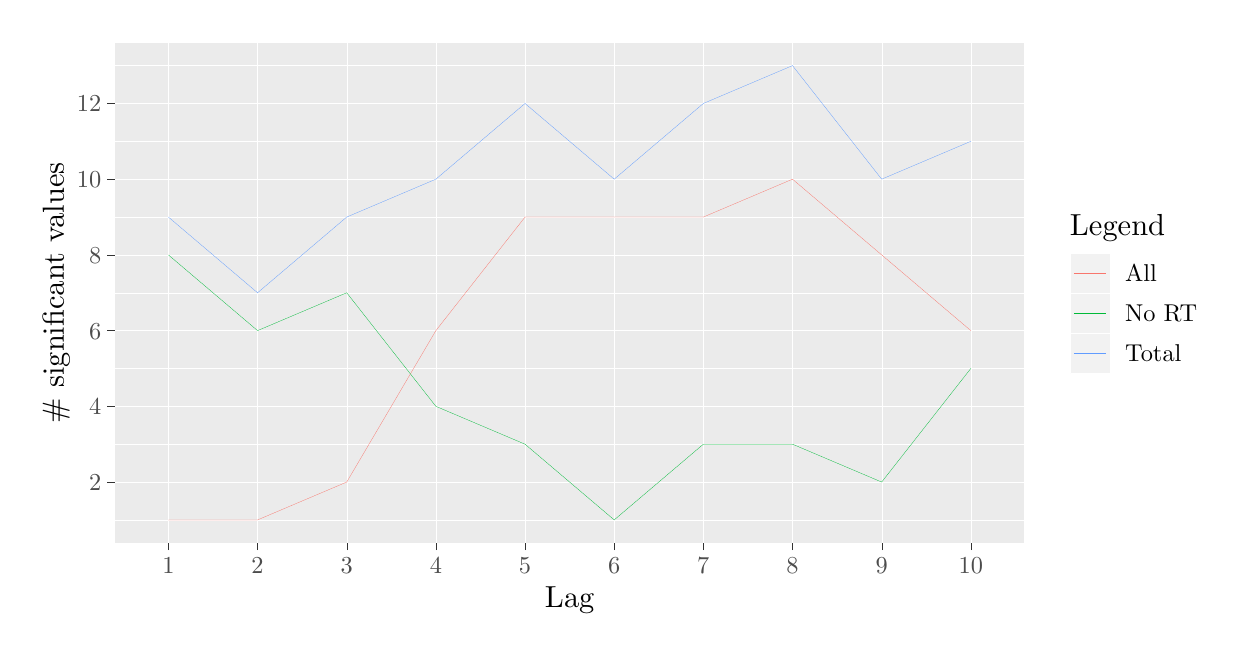
\begin{tikzpicture}[x=1pt,y=1pt]
\definecolor{fillColor}{RGB}{255,255,255}
\path[use as bounding box,fill=fillColor,fill opacity=0.00] (0,0) rectangle (433.62,216.81);
\begin{scope}
\path[clip] (  0.00,  0.00) rectangle (433.62,216.81);
\definecolor{drawColor}{RGB}{255,255,255}
\definecolor{fillColor}{RGB}{255,255,255}

\path[draw=drawColor,line width= 0.1pt,line join=round,line cap=round,fill=fillColor] (  0.00,  0.00) rectangle (433.62,216.81);
\end{scope}
\begin{scope}
\path[clip] ( 31.52, 30.73) rectangle (360.13,211.31);
\definecolor{fillColor}{gray}{0.92}

\path[fill=fillColor] ( 31.52, 30.73) rectangle (360.13,211.31);
\definecolor{drawColor}{RGB}{255,255,255}

\path[draw=drawColor,line width= 0.1pt,line join=round] ( 31.52, 38.94) --
	(360.13, 38.94);

\path[draw=drawColor,line width= 0.1pt,line join=round] ( 31.52, 66.30) --
	(360.13, 66.30);

\path[draw=drawColor,line width= 0.1pt,line join=round] ( 31.52, 93.66) --
	(360.13, 93.66);

\path[draw=drawColor,line width= 0.1pt,line join=round] ( 31.52,121.02) --
	(360.13,121.02);

\path[draw=drawColor,line width= 0.1pt,line join=round] ( 31.52,148.38) --
	(360.13,148.38);

\path[draw=drawColor,line width= 0.1pt,line join=round] ( 31.52,175.74) --
	(360.13,175.74);

\path[draw=drawColor,line width= 0.1pt,line join=round] ( 31.52,203.10) --
	(360.13,203.10);

\path[draw=drawColor,line width= 0.1pt,line join=round] ( 31.52, 52.62) --
	(360.13, 52.62);

\path[draw=drawColor,line width= 0.1pt,line join=round] ( 31.52, 79.98) --
	(360.13, 79.98);

\path[draw=drawColor,line width= 0.1pt,line join=round] ( 31.52,107.34) --
	(360.13,107.34);

\path[draw=drawColor,line width= 0.1pt,line join=round] ( 31.52,134.70) --
	(360.13,134.70);

\path[draw=drawColor,line width= 0.1pt,line join=round] ( 31.52,162.06) --
	(360.13,162.06);

\path[draw=drawColor,line width= 0.1pt,line join=round] ( 31.52,189.42) --
	(360.13,189.42);

\path[draw=drawColor,line width= 0.1pt,line join=round] ( 50.85, 30.73) --
	( 50.85,211.31);

\path[draw=drawColor,line width= 0.1pt,line join=round] ( 83.07, 30.73) --
	( 83.07,211.31);

\path[draw=drawColor,line width= 0.1pt,line join=round] (115.29, 30.73) --
	(115.29,211.31);

\path[draw=drawColor,line width= 0.1pt,line join=round] (147.50, 30.73) --
	(147.50,211.31);

\path[draw=drawColor,line width= 0.1pt,line join=round] (179.72, 30.73) --
	(179.72,211.31);

\path[draw=drawColor,line width= 0.1pt,line join=round] (211.94, 30.73) --
	(211.94,211.31);

\path[draw=drawColor,line width= 0.1pt,line join=round] (244.15, 30.73) --
	(244.15,211.31);

\path[draw=drawColor,line width= 0.1pt,line join=round] (276.37, 30.73) --
	(276.37,211.31);

\path[draw=drawColor,line width= 0.1pt,line join=round] (308.59, 30.73) --
	(308.59,211.31);

\path[draw=drawColor,line width= 0.1pt,line join=round] (340.80, 30.73) --
	(340.80,211.31);
\definecolor{drawColor}{RGB}{248,118,109}

\path[draw=drawColor,line width= 0.1pt,line join=round] ( 50.85, 38.94) --
	( 83.07, 38.94) --
	(115.29, 52.62) --
	(147.50,107.34) --
	(179.72,148.38) --
	(211.94,148.38) --
	(244.15,148.38) --
	(276.37,162.06) --
	(308.59,134.70) --
	(340.80,107.34);
\definecolor{drawColor}{RGB}{0,186,56}

\path[draw=drawColor,line width= 0.1pt,line join=round] ( 50.85,134.70) --
	( 83.07,107.34) --
	(115.29,121.02) --
	(147.50, 79.98) --
	(179.72, 66.30) --
	(211.94, 38.94) --
	(244.15, 66.30) --
	(276.37, 66.30) --
	(308.59, 52.62) --
	(340.80, 93.66);
\definecolor{drawColor}{RGB}{97,156,255}

\path[draw=drawColor,line width= 0.1pt,line join=round] ( 50.85,148.38) --
	( 83.07,121.02) --
	(115.29,148.38) --
	(147.50,162.06) --
	(179.72,189.42) --
	(211.94,162.06) --
	(244.15,189.42) --
	(276.37,203.10) --
	(308.59,162.06) --
	(340.80,175.74);
\end{scope}
\begin{scope}
\path[clip] (  0.00,  0.00) rectangle (433.62,216.81);
\definecolor{drawColor}{gray}{0.30}

\node[text=drawColor,anchor=base east,inner sep=0pt, outer sep=0pt, scale=  0.88] at ( 26.57, 49.59) {2};

\node[text=drawColor,anchor=base east,inner sep=0pt, outer sep=0pt, scale=  0.88] at ( 26.57, 76.95) {4};

\node[text=drawColor,anchor=base east,inner sep=0pt, outer sep=0pt, scale=  0.88] at ( 26.57,104.31) {6};

\node[text=drawColor,anchor=base east,inner sep=0pt, outer sep=0pt, scale=  0.88] at ( 26.57,131.67) {8};

\node[text=drawColor,anchor=base east,inner sep=0pt, outer sep=0pt, scale=  0.88] at ( 26.57,159.03) {10};

\node[text=drawColor,anchor=base east,inner sep=0pt, outer sep=0pt, scale=  0.88] at ( 26.57,186.39) {12};
\end{scope}
\begin{scope}
\path[clip] (  0.00,  0.00) rectangle (433.62,216.81);
\definecolor{drawColor}{gray}{0.20}

\path[draw=drawColor,line width= 0.1pt,line join=round] ( 28.77, 52.62) --
	( 31.52, 52.62);

\path[draw=drawColor,line width= 0.1pt,line join=round] ( 28.77, 79.98) --
	( 31.52, 79.98);

\path[draw=drawColor,line width= 0.1pt,line join=round] ( 28.77,107.34) --
	( 31.52,107.34);

\path[draw=drawColor,line width= 0.1pt,line join=round] ( 28.77,134.70) --
	( 31.52,134.70);

\path[draw=drawColor,line width= 0.1pt,line join=round] ( 28.77,162.06) --
	( 31.52,162.06);

\path[draw=drawColor,line width= 0.1pt,line join=round] ( 28.77,189.42) --
	( 31.52,189.42);
\end{scope}
\begin{scope}
\path[clip] (  0.00,  0.00) rectangle (433.62,216.81);
\definecolor{drawColor}{gray}{0.20}

\path[draw=drawColor,line width= 0.1pt,line join=round] ( 50.85, 27.98) --
	( 50.85, 30.73);

\path[draw=drawColor,line width= 0.1pt,line join=round] ( 83.07, 27.98) --
	( 83.07, 30.73);

\path[draw=drawColor,line width= 0.1pt,line join=round] (115.29, 27.98) --
	(115.29, 30.73);

\path[draw=drawColor,line width= 0.1pt,line join=round] (147.50, 27.98) --
	(147.50, 30.73);

\path[draw=drawColor,line width= 0.1pt,line join=round] (179.72, 27.98) --
	(179.72, 30.73);

\path[draw=drawColor,line width= 0.1pt,line join=round] (211.94, 27.98) --
	(211.94, 30.73);

\path[draw=drawColor,line width= 0.1pt,line join=round] (244.15, 27.98) --
	(244.15, 30.73);

\path[draw=drawColor,line width= 0.1pt,line join=round] (276.37, 27.98) --
	(276.37, 30.73);

\path[draw=drawColor,line width= 0.1pt,line join=round] (308.59, 27.98) --
	(308.59, 30.73);

\path[draw=drawColor,line width= 0.1pt,line join=round] (340.80, 27.98) --
	(340.80, 30.73);
\end{scope}
\begin{scope}
\path[clip] (  0.00,  0.00) rectangle (433.62,216.81);
\definecolor{drawColor}{gray}{0.30}

\node[text=drawColor,anchor=base,inner sep=0pt, outer sep=0pt, scale=  0.88] at ( 50.85, 19.72) { 1};

\node[text=drawColor,anchor=base,inner sep=0pt, outer sep=0pt, scale=  0.88] at ( 83.07, 19.72) { 2};

\node[text=drawColor,anchor=base,inner sep=0pt, outer sep=0pt, scale=  0.88] at (115.29, 19.72) { 3};

\node[text=drawColor,anchor=base,inner sep=0pt, outer sep=0pt, scale=  0.88] at (147.50, 19.72) { 4};

\node[text=drawColor,anchor=base,inner sep=0pt, outer sep=0pt, scale=  0.88] at (179.72, 19.72) { 5};

\node[text=drawColor,anchor=base,inner sep=0pt, outer sep=0pt, scale=  0.88] at (211.94, 19.72) { 6};

\node[text=drawColor,anchor=base,inner sep=0pt, outer sep=0pt, scale=  0.88] at (244.15, 19.72) { 7};

\node[text=drawColor,anchor=base,inner sep=0pt, outer sep=0pt, scale=  0.88] at (276.37, 19.72) { 8};

\node[text=drawColor,anchor=base,inner sep=0pt, outer sep=0pt, scale=  0.88] at (308.59, 19.72) { 9};

\node[text=drawColor,anchor=base,inner sep=0pt, outer sep=0pt, scale=  0.88] at (340.80, 19.72) {10};
\end{scope}
\begin{scope}
\path[clip] (  0.00,  0.00) rectangle (433.62,216.81);
\definecolor{drawColor}{RGB}{0,0,0}

\node[text=drawColor,anchor=base,inner sep=0pt, outer sep=0pt, scale=  1.10] at (195.83,  7.44) {Lag};
\end{scope}
\begin{scope}
\path[clip] (  0.00,  0.00) rectangle (433.62,216.81);
\definecolor{drawColor}{RGB}{0,0,0}

\node[text=drawColor,rotate= 90.00,anchor=base,inner sep=0pt, outer sep=0pt, scale=  1.10] at ( 13.08,121.02) {\# significant values};
\end{scope}
\begin{scope}
\path[clip] (  0.00,  0.00) rectangle (433.62,216.81);
\definecolor{fillColor}{RGB}{255,255,255}

\path[fill=fillColor] (371.13, 86.33) rectangle (428.12,155.71);
\end{scope}
\begin{scope}
\path[clip] (  0.00,  0.00) rectangle (433.62,216.81);
\definecolor{drawColor}{RGB}{0,0,0}

\node[text=drawColor,anchor=base west,inner sep=0pt, outer sep=0pt, scale=  1.10] at (376.63,141.66) {Legend};
\end{scope}
\begin{scope}
\path[clip] (  0.00,  0.00) rectangle (433.62,216.81);
\definecolor{drawColor}{RGB}{255,255,255}
\definecolor{fillColor}{gray}{0.95}

\path[draw=drawColor,line width= 0.1pt,line join=round,line cap=round,fill=fillColor] (376.63,120.74) rectangle (391.09,135.19);
\end{scope}
\begin{scope}
\path[clip] (  0.00,  0.00) rectangle (433.62,216.81);
\definecolor{drawColor}{RGB}{248,118,109}

\path[draw=drawColor,line width= 0.1pt,line join=round] (378.08,127.96) -- (389.64,127.96);
\end{scope}
\begin{scope}
\path[clip] (  0.00,  0.00) rectangle (433.62,216.81);
\definecolor{drawColor}{RGB}{255,255,255}
\definecolor{fillColor}{gray}{0.95}

\path[draw=drawColor,line width= 0.1pt,line join=round,line cap=round,fill=fillColor] (376.63,106.28) rectangle (391.09,120.74);
\end{scope}
\begin{scope}
\path[clip] (  0.00,  0.00) rectangle (433.62,216.81);
\definecolor{drawColor}{RGB}{0,186,56}

\path[draw=drawColor,line width= 0.1pt,line join=round] (378.08,113.51) -- (389.64,113.51);
\end{scope}
\begin{scope}
\path[clip] (  0.00,  0.00) rectangle (433.62,216.81);
\definecolor{drawColor}{RGB}{255,255,255}
\definecolor{fillColor}{gray}{0.95}

\path[draw=drawColor,line width= 0.1pt,line join=round,line cap=round,fill=fillColor] (376.63, 91.83) rectangle (391.09,106.28);
\end{scope}
\begin{scope}
\path[clip] (  0.00,  0.00) rectangle (433.62,216.81);
\definecolor{drawColor}{RGB}{97,156,255}

\path[draw=drawColor,line width= 0.1pt,line join=round] (378.08, 99.05) -- (389.64, 99.05);
\end{scope}
\begin{scope}
\path[clip] (  0.00,  0.00) rectangle (433.62,216.81);
\definecolor{drawColor}{RGB}{0,0,0}

\node[text=drawColor,anchor=base west,inner sep=0pt, outer sep=0pt, scale=  0.88] at (396.59,124.93) {All};
\end{scope}
\begin{scope}
\path[clip] (  0.00,  0.00) rectangle (433.62,216.81);
\definecolor{drawColor}{RGB}{0,0,0}

\node[text=drawColor,anchor=base west,inner sep=0pt, outer sep=0pt, scale=  0.88] at (396.59,110.48) {No RT};
\end{scope}
\begin{scope}
\path[clip] (  0.00,  0.00) rectangle (433.62,216.81);
\definecolor{drawColor}{RGB}{0,0,0}

\node[text=drawColor,anchor=base west,inner sep=0pt, outer sep=0pt, scale=  0.88] at (396.59, 96.02) {Total};
\end{scope}
\end{tikzpicture}
